\documentclass[tikz,border=10pt]{standalone}
\usepackage{pgfplots}
\pgfplotsset{compat=1.17}

\begin{document}
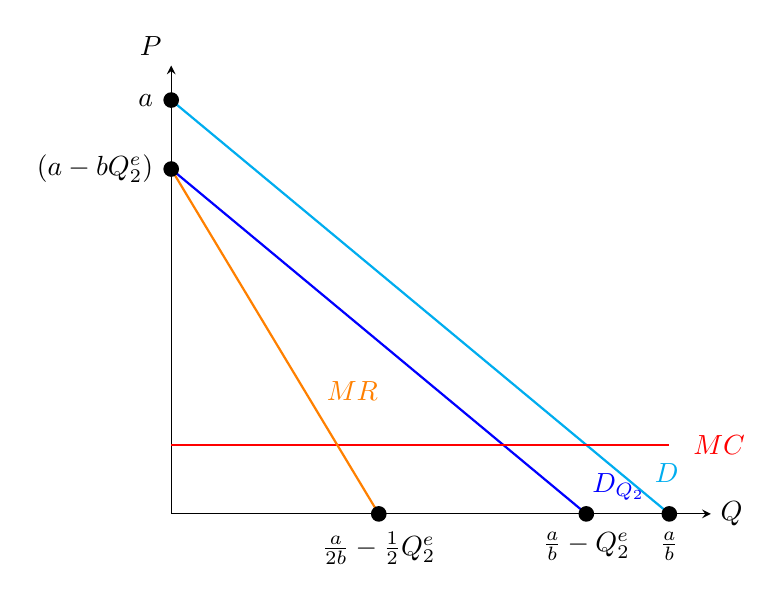
\begin{tikzpicture}
\begin{axis}[
    axis lines=left,
    xlabel={$Q$},
    ylabel={$P$},
    ymin=0, ymax=13,
    xmin=0, xmax=13,
    xtick=\empty, 
    ytick=\empty,
    clip=false,
    xlabel style={at={(ticklabel* cs:1)},anchor=west},
    ylabel style={at={(ticklabel* cs:1)},anchor=south east, rotate=-90},
    every axis plot/.append style={thick},
]

% Demand Line
\addplot[domain=0:12, color=cyan] {12-x} node[pos=.95, anchor=south west] {$D$};
\addplot[domain=0:10, color=blue] {10-x} node[pos=.99, anchor=south west] {$D_{Q_2}$};

% Marginal Cost Line
\addplot[domain=0:12, color=red] {2} node[pos=1.1] {$MC$};

% Marginal Revenue Line
\addplot[domain=0:5, color=orange] {10-2*x} node[pos=0.7, anchor=south west] {$MR$};

% Labels
\node[label={180:{\( a \)}},circle,fill,inner sep=2pt] at (axis cs:0,12) {};
% \node[label={180:{\( P_a \)}},circle,fill,inner sep=2pt] at (axis cs:5,6) {};
\node[label={180:{\( (a-bQ_2^e) \)}},circle,fill,inner sep=2pt] at (axis cs:0,10) {};
\node[label={270:{\( \frac{a}{b} \)}},circle,fill,inner sep=2pt] at (axis cs:12,0) {};
\node[label={270:{\( \frac{a}{2b} - \frac{1}{2}Q_2^e \)}},circle,fill,inner sep=2pt] at (axis cs:5,0) {};
\node[label={270:{\( \frac{a}{b} - Q_2^e \)}},circle,fill,inner sep=2pt] at (axis cs:10,0) {};

\end{axis}
\end{tikzpicture}
\end{document}
